% Options for packages loaded elsewhere
\PassOptionsToPackage{unicode}{hyperref}
\PassOptionsToPackage{hyphens}{url}
%
\documentclass[
]{article}
\usepackage{amsmath,amssymb}
\usepackage{iftex}
\ifPDFTeX
  \usepackage[T1]{fontenc}
  \usepackage[utf8]{inputenc}
  \usepackage{textcomp} % provide euro and other symbols
\else % if luatex or xetex
  \usepackage{unicode-math} % this also loads fontspec
  \defaultfontfeatures{Scale=MatchLowercase}
  \defaultfontfeatures[\rmfamily]{Ligatures=TeX,Scale=1}
\fi
\usepackage{lmodern}
\ifPDFTeX\else
  % xetex/luatex font selection
\fi
% Use upquote if available, for straight quotes in verbatim environments
\IfFileExists{upquote.sty}{\usepackage{upquote}}{}
\IfFileExists{microtype.sty}{% use microtype if available
  \usepackage[]{microtype}
  \UseMicrotypeSet[protrusion]{basicmath} % disable protrusion for tt fonts
}{}
\makeatletter
\@ifundefined{KOMAClassName}{% if non-KOMA class
  \IfFileExists{parskip.sty}{%
    \usepackage{parskip}
  }{% else
    \setlength{\parindent}{0pt}
    \setlength{\parskip}{6pt plus 2pt minus 1pt}}
}{% if KOMA class
  \KOMAoptions{parskip=half}}
\makeatother
\usepackage{xcolor}
\usepackage[margin=1in]{geometry}
\usepackage{color}
\usepackage{fancyvrb}
\newcommand{\VerbBar}{|}
\newcommand{\VERB}{\Verb[commandchars=\\\{\}]}
\DefineVerbatimEnvironment{Highlighting}{Verbatim}{commandchars=\\\{\}}
% Add ',fontsize=\small' for more characters per line
\usepackage{framed}
\definecolor{shadecolor}{RGB}{248,248,248}
\newenvironment{Shaded}{\begin{snugshade}}{\end{snugshade}}
\newcommand{\AlertTok}[1]{\textcolor[rgb]{0.94,0.16,0.16}{#1}}
\newcommand{\AnnotationTok}[1]{\textcolor[rgb]{0.56,0.35,0.01}{\textbf{\textit{#1}}}}
\newcommand{\AttributeTok}[1]{\textcolor[rgb]{0.13,0.29,0.53}{#1}}
\newcommand{\BaseNTok}[1]{\textcolor[rgb]{0.00,0.00,0.81}{#1}}
\newcommand{\BuiltInTok}[1]{#1}
\newcommand{\CharTok}[1]{\textcolor[rgb]{0.31,0.60,0.02}{#1}}
\newcommand{\CommentTok}[1]{\textcolor[rgb]{0.56,0.35,0.01}{\textit{#1}}}
\newcommand{\CommentVarTok}[1]{\textcolor[rgb]{0.56,0.35,0.01}{\textbf{\textit{#1}}}}
\newcommand{\ConstantTok}[1]{\textcolor[rgb]{0.56,0.35,0.01}{#1}}
\newcommand{\ControlFlowTok}[1]{\textcolor[rgb]{0.13,0.29,0.53}{\textbf{#1}}}
\newcommand{\DataTypeTok}[1]{\textcolor[rgb]{0.13,0.29,0.53}{#1}}
\newcommand{\DecValTok}[1]{\textcolor[rgb]{0.00,0.00,0.81}{#1}}
\newcommand{\DocumentationTok}[1]{\textcolor[rgb]{0.56,0.35,0.01}{\textbf{\textit{#1}}}}
\newcommand{\ErrorTok}[1]{\textcolor[rgb]{0.64,0.00,0.00}{\textbf{#1}}}
\newcommand{\ExtensionTok}[1]{#1}
\newcommand{\FloatTok}[1]{\textcolor[rgb]{0.00,0.00,0.81}{#1}}
\newcommand{\FunctionTok}[1]{\textcolor[rgb]{0.13,0.29,0.53}{\textbf{#1}}}
\newcommand{\ImportTok}[1]{#1}
\newcommand{\InformationTok}[1]{\textcolor[rgb]{0.56,0.35,0.01}{\textbf{\textit{#1}}}}
\newcommand{\KeywordTok}[1]{\textcolor[rgb]{0.13,0.29,0.53}{\textbf{#1}}}
\newcommand{\NormalTok}[1]{#1}
\newcommand{\OperatorTok}[1]{\textcolor[rgb]{0.81,0.36,0.00}{\textbf{#1}}}
\newcommand{\OtherTok}[1]{\textcolor[rgb]{0.56,0.35,0.01}{#1}}
\newcommand{\PreprocessorTok}[1]{\textcolor[rgb]{0.56,0.35,0.01}{\textit{#1}}}
\newcommand{\RegionMarkerTok}[1]{#1}
\newcommand{\SpecialCharTok}[1]{\textcolor[rgb]{0.81,0.36,0.00}{\textbf{#1}}}
\newcommand{\SpecialStringTok}[1]{\textcolor[rgb]{0.31,0.60,0.02}{#1}}
\newcommand{\StringTok}[1]{\textcolor[rgb]{0.31,0.60,0.02}{#1}}
\newcommand{\VariableTok}[1]{\textcolor[rgb]{0.00,0.00,0.00}{#1}}
\newcommand{\VerbatimStringTok}[1]{\textcolor[rgb]{0.31,0.60,0.02}{#1}}
\newcommand{\WarningTok}[1]{\textcolor[rgb]{0.56,0.35,0.01}{\textbf{\textit{#1}}}}
\usepackage{graphicx}
\makeatletter
\def\maxwidth{\ifdim\Gin@nat@width>\linewidth\linewidth\else\Gin@nat@width\fi}
\def\maxheight{\ifdim\Gin@nat@height>\textheight\textheight\else\Gin@nat@height\fi}
\makeatother
% Scale images if necessary, so that they will not overflow the page
% margins by default, and it is still possible to overwrite the defaults
% using explicit options in \includegraphics[width, height, ...]{}
\setkeys{Gin}{width=\maxwidth,height=\maxheight,keepaspectratio}
% Set default figure placement to htbp
\makeatletter
\def\fps@figure{htbp}
\makeatother
\setlength{\emergencystretch}{3em} % prevent overfull lines
\providecommand{\tightlist}{%
  \setlength{\itemsep}{0pt}\setlength{\parskip}{0pt}}
\setcounter{secnumdepth}{-\maxdimen} % remove section numbering
\ifLuaTeX
  \usepackage{selnolig}  % disable illegal ligatures
\fi
\IfFileExists{bookmark.sty}{\usepackage{bookmark}}{\usepackage{hyperref}}
\IfFileExists{xurl.sty}{\usepackage{xurl}}{} % add URL line breaks if available
\urlstyle{same}
\hypersetup{
  pdftitle={McDonald's EDA},
  hidelinks,
  pdfcreator={LaTeX via pandoc}}

\title{McDonald's EDA}
\author{}
\date{\vspace{-2.5em}}

\begin{document}
\maketitle

The EDA (Exploratory Data Analysis) on McDonald's data revealed insights
into customers purchasing patterns, and menu preferences. It provides
valuable information for customers to make decisions on their dietary
wants and also valuable information for strategic decision-making and
targeted marketing efforts.

You can download the
\href{https://www.kaggle.com/datasets/mcdonalds/nutrition-facts/data}{dataset
here}

\hypertarget{packages}{%
\section{Packages}\label{packages}}

\emph{Load the Packages for data manipulation and visualization}

\begin{Shaded}
\begin{Highlighting}[]
\FunctionTok{library}\NormalTok{(dplyr)}
\end{Highlighting}
\end{Shaded}

\begin{verbatim}
## 
## Attaching package: 'dplyr'
\end{verbatim}

\begin{verbatim}
## The following objects are masked from 'package:stats':
## 
##     filter, lag
\end{verbatim}

\begin{verbatim}
## The following objects are masked from 'package:base':
## 
##     intersect, setdiff, setequal, union
\end{verbatim}

\begin{Shaded}
\begin{Highlighting}[]
\FunctionTok{library}\NormalTok{(tidyverse)}
\end{Highlighting}
\end{Shaded}

\begin{verbatim}
## -- Attaching core tidyverse packages ------------------------ tidyverse 2.0.0 --
## v forcats   1.0.0     v readr     2.1.5
## v ggplot2   3.5.0     v stringr   1.5.1
## v lubridate 1.9.3     v tibble    3.2.1
## v purrr     1.0.2     v tidyr     1.3.1
\end{verbatim}

\begin{verbatim}
## -- Conflicts ------------------------------------------ tidyverse_conflicts() --
## x dplyr::filter() masks stats::filter()
## x dplyr::lag()    masks stats::lag()
## i Use the conflicted package (<http://conflicted.r-lib.org/>) to force all conflicts to become errors
\end{verbatim}

\begin{Shaded}
\begin{Highlighting}[]
\FunctionTok{library}\NormalTok{(GGally)}
\end{Highlighting}
\end{Shaded}

\begin{verbatim}
## Registered S3 method overwritten by 'GGally':
##   method from   
##   +.gg   ggplot2
\end{verbatim}

\begin{center}\rule{0.5\linewidth}{0.5pt}\end{center}

\emph{Read in the data}

\begin{center}\rule{0.5\linewidth}{0.5pt}\end{center}

\begin{Shaded}
\begin{Highlighting}[]
\NormalTok{menu }\OtherTok{\textless{}{-}} \FunctionTok{read.csv}\NormalTok{(}\StringTok{"menu.csv"}\NormalTok{)}
\end{Highlighting}
\end{Shaded}

\hypertarget{category}{%
\subsubsection{Category}\label{category}}

\begin{center}\rule{0.5\linewidth}{0.5pt}\end{center}

The Menu Category is grouped according to the total number food items in
each Category.

\begin{center}\rule{0.5\linewidth}{0.5pt}\end{center}

\begin{Shaded}
\begin{Highlighting}[]
\NormalTok{cat }\OtherTok{\textless{}{-}}\NormalTok{ menu }\SpecialCharTok{\%\textgreater{}\%} 
  \FunctionTok{select}\NormalTok{(Category) }\SpecialCharTok{\%\textgreater{}\%} 
  \FunctionTok{count}\NormalTok{(Category,}\AttributeTok{name =} \StringTok{"Total"}\NormalTok{)  }\SpecialCharTok{\%\textgreater{}\%} 
  \FunctionTok{distinct}\NormalTok{()}

\NormalTok{cat\_plot }\OtherTok{\textless{}{-}}\NormalTok{ cat }\SpecialCharTok{\%\textgreater{}\%} 
  \FunctionTok{ggplot}\NormalTok{(}\FunctionTok{aes}\NormalTok{(Category,}
\NormalTok{             Total,}
             \AttributeTok{fill =}\NormalTok{ Category)) }\SpecialCharTok{+} 
  \FunctionTok{geom\_col}\NormalTok{() }\SpecialCharTok{+} 
  \FunctionTok{theme\_classic}\NormalTok{() }\SpecialCharTok{+} 
  \FunctionTok{labs}\NormalTok{(}\AttributeTok{title =} \StringTok{"Total Categories"}\NormalTok{) }\SpecialCharTok{+} 
  \FunctionTok{theme}\NormalTok{(}\AttributeTok{legend.position =} \StringTok{"none"}\NormalTok{) }\SpecialCharTok{+} 
  \FunctionTok{geom\_text}\NormalTok{(}\FunctionTok{aes}\NormalTok{(}\AttributeTok{label =}\NormalTok{ Total), }
            \AttributeTok{position =} \FunctionTok{position\_stack}\NormalTok{(}\AttributeTok{vjust =} \FloatTok{0.5}\NormalTok{),}
            \AttributeTok{color =}\StringTok{"black"}\NormalTok{, }\AttributeTok{size =} \DecValTok{3}\NormalTok{) }\SpecialCharTok{+} \FunctionTok{coord\_flip}\NormalTok{()}


\NormalTok{cat\_plot}
\end{Highlighting}
\end{Shaded}

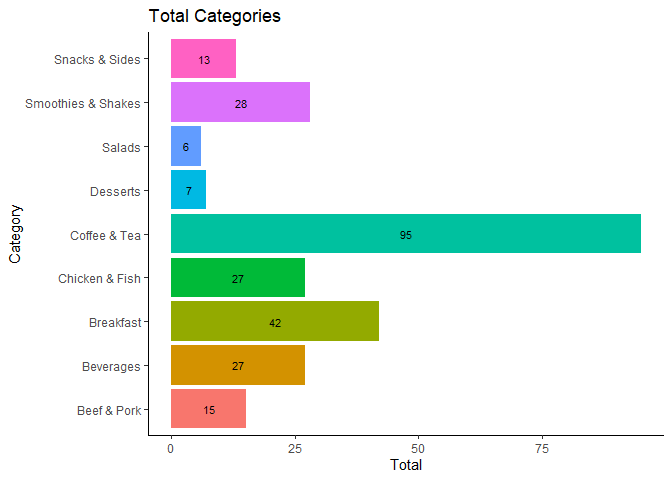
\includegraphics{index_files/figure-latex/unnamed-chunk-3-1.pdf}

\hypertarget{protein}{%
\section{Protein}\label{protein}}

\begin{center}\rule{0.5\linewidth}{0.5pt}\end{center}

Proteins are made up of chemical `building blocks' called amino acids.
Your body uses amino acids to build and repair muscles and bones and to
make hormones and enzymes. They can also be used as an energy source.

\begin{center}\rule{0.5\linewidth}{0.5pt}\end{center}

\hypertarget{the-average-protein-content-in-the-menu-category}{%
\subsubsection{The Average Protein Content in the Menu
Category}\label{the-average-protein-content-in-the-menu-category}}

\begin{Shaded}
\begin{Highlighting}[]
\NormalTok{Pro\_avg }\OtherTok{\textless{}{-}}\NormalTok{ menu }\SpecialCharTok{\%\textgreater{}\%} 
  \FunctionTok{select}\NormalTok{(Category,Item,Protein) }\SpecialCharTok{\%\textgreater{}\%} 
  \FunctionTok{group\_by}\NormalTok{(Category) }\SpecialCharTok{\%\textgreater{}\%}
  \FunctionTok{aggregate}\NormalTok{(Protein}\SpecialCharTok{\textasciitilde{}}\NormalTok{Category, }
            \AttributeTok{FUN =}\NormalTok{ mean)}

\NormalTok{Pro\_avg}
\end{Highlighting}
\end{Shaded}

\begin{verbatim}
##             Category   Protein
## 1        Beef & Pork 27.333333
## 2          Beverages  1.333333
## 3          Breakfast 19.857143
## 4     Chicken & Fish 29.111111
## 5       Coffee & Tea  8.863158
## 6           Desserts  4.000000
## 7             Salads 19.833333
## 8 Smoothies & Shakes 10.857143
## 9     Snacks & Sides  8.384615
\end{verbatim}

\hypertarget{the-menu-item-that-contains-the-highest-amount-of-protein-content}{%
\subsubsection{The Menu item that contains the highest amount of Protein
content}\label{the-menu-item-that-contains-the-highest-amount-of-protein-content}}

\begin{Shaded}
\begin{Highlighting}[]
\NormalTok{max\_pro }\OtherTok{\textless{}{-}}\NormalTok{ menu }\SpecialCharTok{\%\textgreater{}\%} 
  \FunctionTok{select}\NormalTok{(Item,Protein) }\SpecialCharTok{\%\textgreater{}\%}  
  \FunctionTok{group\_by}\NormalTok{(Item) }\SpecialCharTok{\%\textgreater{}\%} 
  \FunctionTok{arrange}\NormalTok{(}\FunctionTok{desc}\NormalTok{(Protein)) }\SpecialCharTok{\%\textgreater{}\%} 
  \FunctionTok{head}\NormalTok{(}\DecValTok{15}\NormalTok{) }\SpecialCharTok{\%\textgreater{}\%} 
  \FunctionTok{ggplot}\NormalTok{(}\FunctionTok{aes}\NormalTok{(}\AttributeTok{x=} \FunctionTok{reorder}\NormalTok{(Item, }
\NormalTok{                        Protein),}
             \AttributeTok{fill =}\NormalTok{ Item)) }\SpecialCharTok{+} 
  \FunctionTok{geom\_bar}\NormalTok{(}\AttributeTok{stat =} \StringTok{"identity"}\NormalTok{,}
           \FunctionTok{aes}\NormalTok{(}\AttributeTok{y=}\NormalTok{ Protein )) }\SpecialCharTok{+}
  \FunctionTok{coord\_flip}\NormalTok{() }\SpecialCharTok{+}
  \FunctionTok{theme\_bw}\NormalTok{()}\SpecialCharTok{+} 
  \FunctionTok{geom\_text}\NormalTok{(}\FunctionTok{aes}\NormalTok{(}\AttributeTok{label =}\NormalTok{ Protein, }
                \AttributeTok{y=}\NormalTok{ Protein),}
            \AttributeTok{position =} \FunctionTok{position\_stack}\NormalTok{(}\AttributeTok{vjust =} \FloatTok{0.5}\NormalTok{),}
            \AttributeTok{color =} \StringTok{"Black"}\NormalTok{,}
            \AttributeTok{size =} \DecValTok{3}\NormalTok{)}\SpecialCharTok{+}
  \FunctionTok{theme}\NormalTok{(}\AttributeTok{legend.position=}\StringTok{"none"}\NormalTok{) }\SpecialCharTok{+}
  \FunctionTok{ggtitle}\NormalTok{(}\StringTok{"TOP 15 McDonald\textquotesingle{}s Menu Item with the Highest Protein Content"}\NormalTok{) }\SpecialCharTok{+}\FunctionTok{theme}\NormalTok{(}\AttributeTok{panel.grid.major =} \FunctionTok{element\_blank}\NormalTok{(), }\AttributeTok{panel.grid.minor =} \FunctionTok{element\_blank}\NormalTok{())}

\NormalTok{max\_pro}
\end{Highlighting}
\end{Shaded}

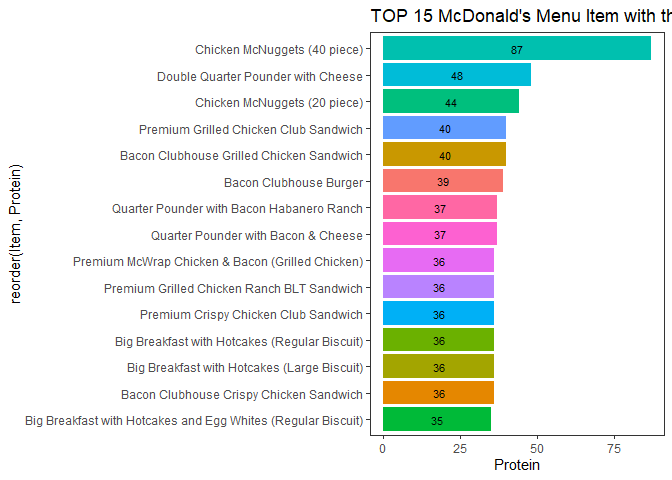
\includegraphics{index_files/figure-latex/unnamed-chunk-5-1.pdf}

\hypertarget{what-menu-item-that-contains-the-least-amount-of-protein-content}{%
\subsubsection{What Menu item that contains the least amount of Protein
content}\label{what-menu-item-that-contains-the-least-amount-of-protein-content}}

\begin{Shaded}
\begin{Highlighting}[]
\NormalTok{min\_pro }\OtherTok{\textless{}{-}}\NormalTok{ menu }\SpecialCharTok{\%\textgreater{}\%} 
  \FunctionTok{select}\NormalTok{(Item,Protein) }\SpecialCharTok{\%\textgreater{}\%}  
  \FunctionTok{group\_by}\NormalTok{(Item, Protein) }\SpecialCharTok{\%\textgreater{}\%} 
  \FunctionTok{filter}\NormalTok{(Protein }\SpecialCharTok{\textgreater{}}\DecValTok{0}\NormalTok{ )}\SpecialCharTok{\%\textgreater{}\%} 
  \FunctionTok{arrange}\NormalTok{(Protein) }\SpecialCharTok{\%\textgreater{}\%} 
  \FunctionTok{head}\NormalTok{(}\DecValTok{15}\NormalTok{)  }\SpecialCharTok{\%\textgreater{}\%} 
  \FunctionTok{ggplot}\NormalTok{(}\FunctionTok{aes}\NormalTok{(}\AttributeTok{x=} \FunctionTok{reorder}\NormalTok{(Item, }
\NormalTok{                        Protein),}
             \AttributeTok{fill =}\NormalTok{ Item)) }\SpecialCharTok{+} 
  \FunctionTok{geom\_bar}\NormalTok{(}\AttributeTok{stat =} \StringTok{"identity"}\NormalTok{,}
           \FunctionTok{aes}\NormalTok{(}\AttributeTok{y=}\NormalTok{ Protein )) }\SpecialCharTok{+}
  \FunctionTok{coord\_flip}\NormalTok{() }\SpecialCharTok{+}
  \FunctionTok{theme\_bw}\NormalTok{()}\SpecialCharTok{+} 
  \FunctionTok{geom\_text}\NormalTok{(}\FunctionTok{aes}\NormalTok{(}\AttributeTok{label =}\NormalTok{ Protein, }
                \AttributeTok{y=}\NormalTok{ Protein),}
            \AttributeTok{position =} \FunctionTok{position\_stack}\NormalTok{(}\AttributeTok{vjust =} \FloatTok{0.5}\NormalTok{),}
            \AttributeTok{color =} \StringTok{"Black"}\NormalTok{,}
            \AttributeTok{size =} \DecValTok{3}\NormalTok{)}\SpecialCharTok{+}
  \FunctionTok{ggtitle}\NormalTok{(}\StringTok{"TOP 10 McDonald\textquotesingle{}s Menu Item with the Least Protein"}\NormalTok{)}\SpecialCharTok{+}
  \FunctionTok{theme}\NormalTok{(}\AttributeTok{legend.position=}\StringTok{"none"}\NormalTok{)}

\NormalTok{min\_pro}
\end{Highlighting}
\end{Shaded}

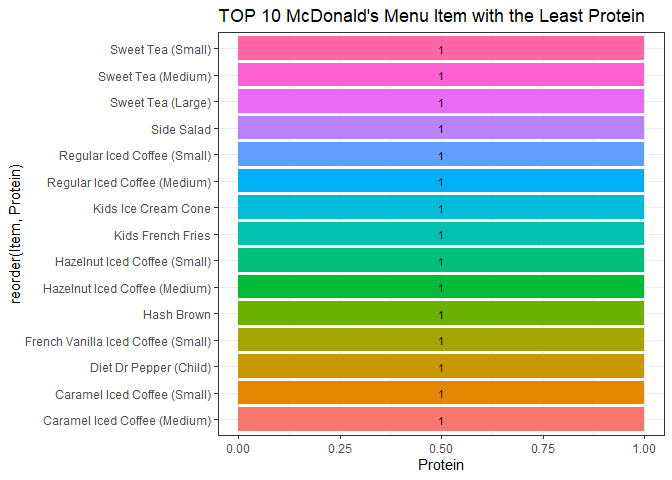
\includegraphics{index_files/figure-latex/unnamed-chunk-6-1.pdf}

\hypertarget{calories}{%
\section{Calories}\label{calories}}

\begin{center}\rule{0.5\linewidth}{0.5pt}\end{center}

A calorie is a measure of energy. Foods have calories. That is, foods
supply the body with energy, which is released when foods are broken
down during digestion. Energy enables cells to do all of their
functions, including building proteins and other substances needed by
the body. The energy can be used immediately or stored for use later.

\begin{center}\rule{0.5\linewidth}{0.5pt}\end{center}

\hypertarget{the-menu-category-ranked-according-to-their-calorie-content}{%
\subsubsection{The Menu Category ranked according to their Calorie
Content}\label{the-menu-category-ranked-according-to-their-calorie-content}}

\begin{Shaded}
\begin{Highlighting}[]
\NormalTok{cal }\OtherTok{\textless{}{-}}\NormalTok{ menu }\SpecialCharTok{\%\textgreater{}\%} 
  \FunctionTok{select}\NormalTok{(Category,}
\NormalTok{         Item,}
\NormalTok{         Calories) }\SpecialCharTok{\%\textgreater{}\%} 
  \FunctionTok{group\_by}\NormalTok{(Category)  }



\NormalTok{cal\_plot }\OtherTok{\textless{}{-}}\NormalTok{ cal }\SpecialCharTok{\%\textgreater{}\%} 
  \FunctionTok{ggplot}\NormalTok{(}\FunctionTok{aes}\NormalTok{(Calories,}
\NormalTok{             Category,}
             \AttributeTok{fill =}\NormalTok{ Category)) }\SpecialCharTok{+} 
  \FunctionTok{geom\_boxplot}\NormalTok{() }\SpecialCharTok{+} 
  \FunctionTok{theme\_classic}\NormalTok{() }\SpecialCharTok{+} 
  \FunctionTok{scale\_fill\_brewer}\NormalTok{(}\AttributeTok{palette =} \StringTok{"Set1"}\NormalTok{) }\SpecialCharTok{+} \FunctionTok{ggtitle}\NormalTok{(}\StringTok{"Calorie Content per Menu Category"}\NormalTok{)}

\NormalTok{cal\_plot}
\end{Highlighting}
\end{Shaded}

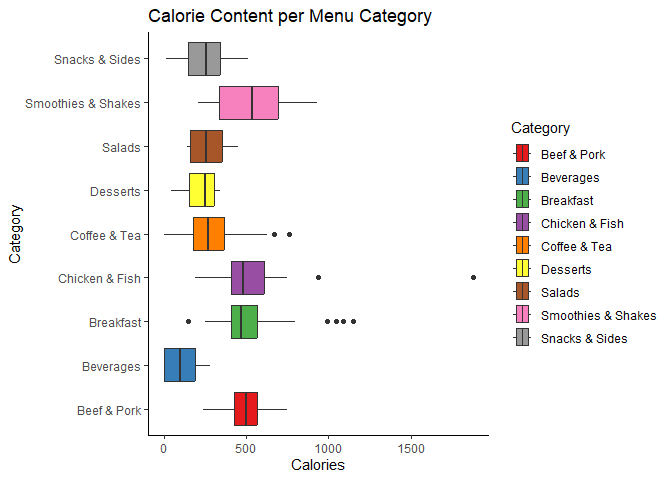
\includegraphics{index_files/figure-latex/unnamed-chunk-7-1.pdf}

\hypertarget{the-top-10-menu-food-items-with-high-calories-content}{%
\subsubsection{The Top 10 Menu Food items with High calories
Content}\label{the-top-10-menu-food-items-with-high-calories-content}}

\begin{Shaded}
\begin{Highlighting}[]
\NormalTok{max\_cal }\OtherTok{\textless{}{-}}\NormalTok{ menu }\SpecialCharTok{\%\textgreater{}\%} 
  \FunctionTok{select}\NormalTok{(Category,}
\NormalTok{         Item,}
\NormalTok{         Calories) }\SpecialCharTok{\%\textgreater{}\%} 
  \FunctionTok{group\_by}\NormalTok{(Item) }\SpecialCharTok{\%\textgreater{}\%} 
  \FunctionTok{arrange}\NormalTok{(}\FunctionTok{desc}\NormalTok{(Calories))}\SpecialCharTok{\%\textgreater{}\%} 
  \FunctionTok{head}\NormalTok{(}\DecValTok{10}\NormalTok{)}\SpecialCharTok{\%\textgreater{}\%} 
  \FunctionTok{ggplot}\NormalTok{(}\FunctionTok{aes}\NormalTok{(Calories,}
             \AttributeTok{y =} \FunctionTok{reorder}\NormalTok{(Item,}
\NormalTok{                         Calories)}
\NormalTok{             ,}\AttributeTok{fill =}\NormalTok{Item)) }\SpecialCharTok{+} 
  \FunctionTok{geom\_col}\NormalTok{() }\SpecialCharTok{+}
  \FunctionTok{theme\_classic}\NormalTok{()}\SpecialCharTok{+}
  \FunctionTok{theme}\NormalTok{(}\AttributeTok{legend.position =} \StringTok{"none"}\NormalTok{) }\SpecialCharTok{+} 
  \FunctionTok{geom\_text}\NormalTok{(}\FunctionTok{aes}\NormalTok{(}\AttributeTok{label =}\NormalTok{ Calories), }
            \AttributeTok{position =} \FunctionTok{position\_stack}\NormalTok{(}\AttributeTok{vjust =} \FloatTok{0.5}\NormalTok{),}
            \AttributeTok{color=}\StringTok{"black"}\NormalTok{, }\AttributeTok{size =}\DecValTok{3}\NormalTok{) }\SpecialCharTok{+} \FunctionTok{ggtitle}\NormalTok{(}\StringTok{"TOP 10 McDonald\textquotesingle{}s Menu Item with the Highest Calorie Content"}\NormalTok{)}

\NormalTok{max\_cal}
\end{Highlighting}
\end{Shaded}

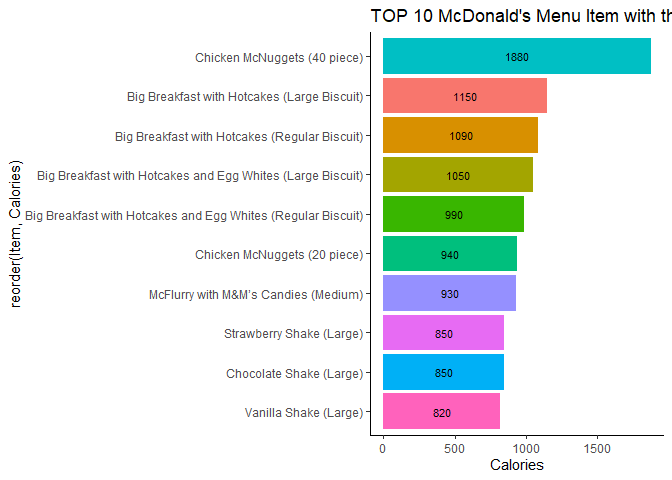
\includegraphics{index_files/figure-latex/unnamed-chunk-8-1.pdf}

\hypertarget{the-top-10-menu-food-items-with-low-calories-content}{%
\subsubsection{The Top 10 Menu Food items with Low calories
Content}\label{the-top-10-menu-food-items-with-low-calories-content}}

\begin{Shaded}
\begin{Highlighting}[]
\NormalTok{min\_cal }\OtherTok{\textless{}{-}}\NormalTok{ menu }\SpecialCharTok{\%\textgreater{}\%}
  \FunctionTok{select}\NormalTok{(Category,}
\NormalTok{         Item,}
\NormalTok{         Calories)}\SpecialCharTok{\%\textgreater{}\%} 
  \FunctionTok{filter}\NormalTok{(Calories}\SpecialCharTok{\textgreater{}}\DecValTok{0}\NormalTok{) }\SpecialCharTok{\%\textgreater{}\%} 
  \FunctionTok{group\_by}\NormalTok{(Item) }\SpecialCharTok{\%\textgreater{}\%} 
  \FunctionTok{arrange}\NormalTok{(Calories)}\SpecialCharTok{\%\textgreater{}\%} 
  \FunctionTok{head}\NormalTok{(}\DecValTok{10}\NormalTok{) }\SpecialCharTok{\%\textgreater{}\%} 
  \FunctionTok{ggplot}\NormalTok{(}\FunctionTok{aes}\NormalTok{(Calories,}
             \AttributeTok{y =} \FunctionTok{reorder}\NormalTok{(Item,}
\NormalTok{                         Calories),}
             \AttributeTok{fill =}\NormalTok{Item)) }\SpecialCharTok{+} 
  \FunctionTok{geom\_col}\NormalTok{() }\SpecialCharTok{+} 
  \FunctionTok{theme\_classic}\NormalTok{()}\SpecialCharTok{+} 
  \FunctionTok{theme}\NormalTok{(}\AttributeTok{legend.position =} \StringTok{"none"}\NormalTok{) }\SpecialCharTok{+} 
  \FunctionTok{geom\_text}\NormalTok{(}\FunctionTok{aes}\NormalTok{(}\AttributeTok{label =}\NormalTok{ Calories), }
            \AttributeTok{position =} \FunctionTok{position\_stack}\NormalTok{(}\AttributeTok{vjust =} \FloatTok{0.5}\NormalTok{),}
            \AttributeTok{color=}\StringTok{"black"}\NormalTok{, }\AttributeTok{size =}\DecValTok{3}\NormalTok{) }\SpecialCharTok{+}
  \FunctionTok{scale\_fill\_brewer}\NormalTok{(}\AttributeTok{palette =} \StringTok{"Set3"}\NormalTok{) }\SpecialCharTok{+} \FunctionTok{ggtitle}\NormalTok{(}\StringTok{"TOP 10 McDonald\textquotesingle{}s Menu Item with Low Calorie Content"}\NormalTok{)}

\NormalTok{min\_cal}
\end{Highlighting}
\end{Shaded}

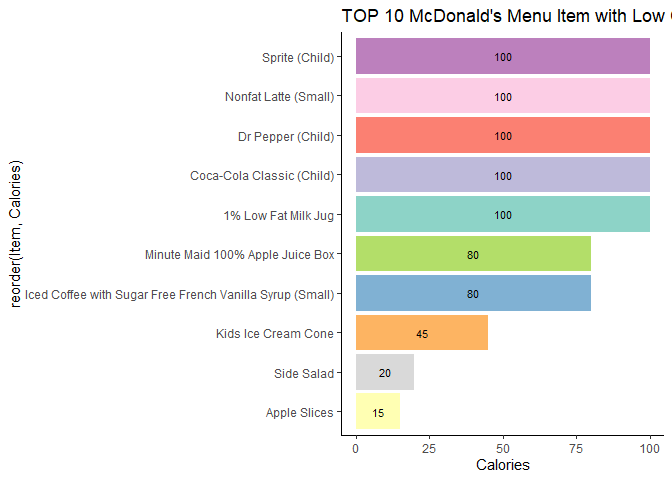
\includegraphics{index_files/figure-latex/unnamed-chunk-9-1.pdf}

\hypertarget{carboydrates}{%
\section{Carboydrates}\label{carboydrates}}

\begin{center}\rule{0.5\linewidth}{0.5pt}\end{center}

Carbohydrates, or carbs, are the sugars, starches, and dietary fiber
that occur in certain foods. The body breaks them down into glucose,
which provides energy.

\begin{center}\rule{0.5\linewidth}{0.5pt}\end{center}

\hypertarget{the-menu-category-with-the-highest-carbohydrates-content}{%
\subsubsection{The Menu Category with the Highest Carbohydrates
Content}\label{the-menu-category-with-the-highest-carbohydrates-content}}

\begin{Shaded}
\begin{Highlighting}[]
\NormalTok{carb }\OtherTok{\textless{}{-}}\NormalTok{ menu }\SpecialCharTok{\%\textgreater{}\%} 
  \FunctionTok{select}\NormalTok{(Category,}
\NormalTok{         Item,}
\NormalTok{         Carbohydrates)}\SpecialCharTok{\%\textgreater{}\%} 
  \FunctionTok{group\_by}\NormalTok{(Category) }

\NormalTok{carb\_plot}\OtherTok{\textless{}{-}}\NormalTok{ carb }\SpecialCharTok{\%\textgreater{}\%}
  \FunctionTok{ggplot}\NormalTok{(}\FunctionTok{aes}\NormalTok{(Category,Carbohydrates, }
             \AttributeTok{fill =}\NormalTok{ Category)) }\SpecialCharTok{+} 
  \FunctionTok{geom\_boxplot}\NormalTok{() }\SpecialCharTok{+}
  \FunctionTok{scale\_fill\_brewer}\NormalTok{(}\AttributeTok{palette =} \StringTok{"Set1"}\NormalTok{) }\SpecialCharTok{+} \FunctionTok{coord\_flip}\NormalTok{() }\SpecialCharTok{+} \FunctionTok{theme\_classic}\NormalTok{() }\SpecialCharTok{+} \FunctionTok{ggtitle}\NormalTok{(}\StringTok{"Menu Category with the Highest Carbohydrates Content"}\NormalTok{)}

\NormalTok{carb\_plot}
\end{Highlighting}
\end{Shaded}

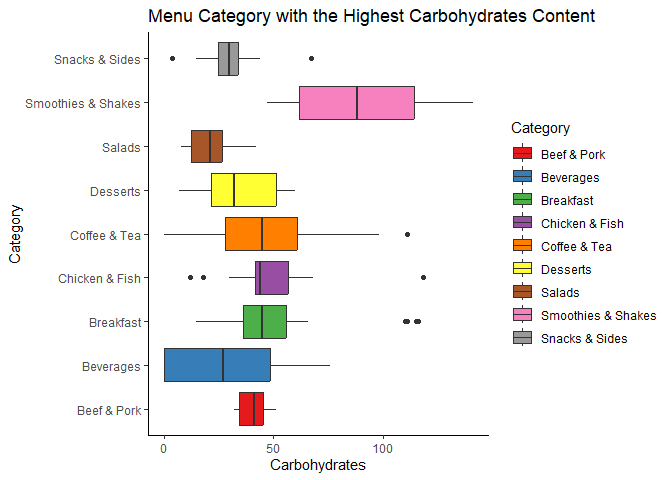
\includegraphics{index_files/figure-latex/unnamed-chunk-10-1.pdf}

\hypertarget{sugar}{%
\subsection{Sugar}\label{sugar}}

\begin{center}\rule{0.5\linewidth}{0.5pt}\end{center}

Sugar also called simple carbohydrates occur naturally in foods, such as
dairy products, as well as added sugar, which are common in baked goods,
sweets, and desserts. The body very easily digests and absorbs sugar.

\begin{center}\rule{0.5\linewidth}{0.5pt}\end{center}

\hypertarget{the-top-10-menu-food-items-with-high-sugar-content}{%
\subsubsection{The Top 10 Menu Food items with High Sugar
Content}\label{the-top-10-menu-food-items-with-high-sugar-content}}

\begin{Shaded}
\begin{Highlighting}[]
\NormalTok{sugar }\OtherTok{\textless{}{-}}\NormalTok{ menu }\SpecialCharTok{\%\textgreater{}\%}
  \FunctionTok{select}\NormalTok{(Category,Item,Sugars) }\SpecialCharTok{\%\textgreater{}\%} 
  \FunctionTok{group\_by}\NormalTok{(Category)}

\NormalTok{max\_sugar }\OtherTok{\textless{}{-}}\NormalTok{sugar }\SpecialCharTok{\%\textgreater{}\%} 
  \FunctionTok{arrange}\NormalTok{(}\FunctionTok{desc}\NormalTok{(Sugars)) }\SpecialCharTok{\%\textgreater{}\%} 
  \FunctionTok{head}\NormalTok{(}\DecValTok{10}\NormalTok{) }\SpecialCharTok{\%\textgreater{}\%} 
  \FunctionTok{ggplot}\NormalTok{(}\FunctionTok{aes}\NormalTok{(Sugars,}
             \AttributeTok{y=}\FunctionTok{reorder}\NormalTok{(Item,}
\NormalTok{                       Sugars),}
             \AttributeTok{fill =}\NormalTok{ Sugars)) }\SpecialCharTok{+}
  \FunctionTok{geom\_col}\NormalTok{() }\SpecialCharTok{+} 
  \FunctionTok{theme\_classic}\NormalTok{()}\SpecialCharTok{+}
  \FunctionTok{theme}\NormalTok{(}\AttributeTok{legend.position =} \StringTok{"none"}\NormalTok{) }\SpecialCharTok{+}
  \FunctionTok{geom\_text}\NormalTok{(}\FunctionTok{aes}\NormalTok{(}\AttributeTok{label =}\NormalTok{ Sugars),}
            \AttributeTok{position =} \FunctionTok{position\_stack}\NormalTok{(}\AttributeTok{vjust =} \FloatTok{0.5}\NormalTok{)) }\SpecialCharTok{+} \FunctionTok{ggtitle}\NormalTok{(}\StringTok{"Top 10 Menu items with the Highest Sugar Content"}\NormalTok{)}


\NormalTok{max\_sugar}
\end{Highlighting}
\end{Shaded}

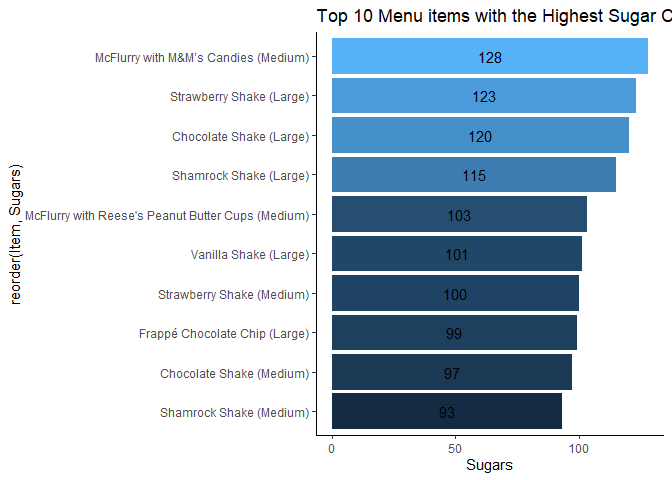
\includegraphics{index_files/figure-latex/unnamed-chunk-11-1.pdf}

\hypertarget{the-top-10-menu-food-items-with-low-sugar-content}{%
\subsubsection{The Top 10 Menu Food items with Low Sugar
Content}\label{the-top-10-menu-food-items-with-low-sugar-content}}

\begin{Shaded}
\begin{Highlighting}[]
\NormalTok{min\_sugar }\OtherTok{\textless{}{-}}\NormalTok{ sugar }\SpecialCharTok{\%\textgreater{}\%} 
  \FunctionTok{filter}\NormalTok{(Sugars}\SpecialCharTok{\textgreater{}}\DecValTok{0}\NormalTok{) }\SpecialCharTok{\%\textgreater{}\%} 
  \FunctionTok{arrange}\NormalTok{(Sugars) }\SpecialCharTok{\%\textgreater{}\%} 
  \FunctionTok{head}\NormalTok{(}\DecValTok{10}\NormalTok{) }\SpecialCharTok{\%\textgreater{}\%} 
  \FunctionTok{ggplot}\NormalTok{(}\FunctionTok{aes}\NormalTok{(Sugars, }
             \AttributeTok{y=}\FunctionTok{reorder}\NormalTok{(Item,}
\NormalTok{                       Sugars),}
             \AttributeTok{fill =}\NormalTok{ Sugars)) }\SpecialCharTok{+}
  \FunctionTok{geom\_col}\NormalTok{() }\SpecialCharTok{+} 
  \FunctionTok{theme\_classic}\NormalTok{()}\SpecialCharTok{+}
  \FunctionTok{theme}\NormalTok{(}\AttributeTok{legend.position =} \StringTok{"none"}\NormalTok{) }\SpecialCharTok{+} 
  \FunctionTok{geom\_text}\NormalTok{(}\FunctionTok{aes}\NormalTok{(}\AttributeTok{label =}\NormalTok{ Sugars),}
            \AttributeTok{position =} \FunctionTok{position\_stack}\NormalTok{(}\AttributeTok{vjust =} \FloatTok{0.5}\NormalTok{)) }\SpecialCharTok{+} \FunctionTok{ggtitle}\NormalTok{(}\StringTok{"Top 10 Menu items with the Lowest sugar Content"}\NormalTok{)}


\NormalTok{min\_sugar}
\end{Highlighting}
\end{Shaded}

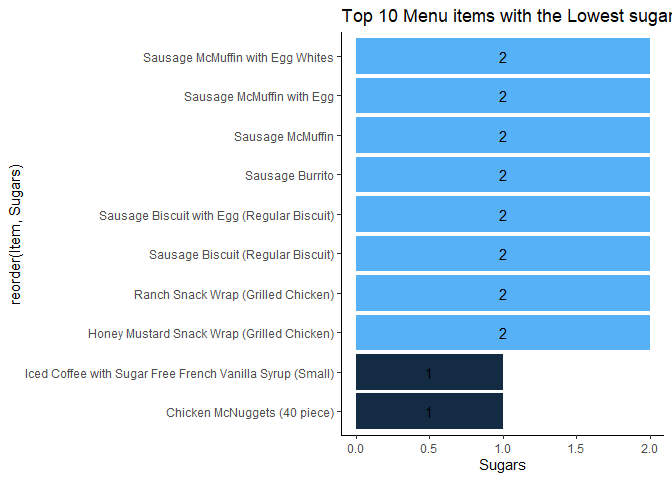
\includegraphics{index_files/figure-latex/unnamed-chunk-12-1.pdf}

\hypertarget{the-menu-categories-with-carbohydrates-that-have-a-higher-fibre-to-sugar-ratiohealthy-carbs}{%
\subsubsection{The Menu Categories with Carbohydrates that have a higher
Fibre to Sugar Ratio(Healthy
Carbs)}\label{the-menu-categories-with-carbohydrates-that-have-a-higher-fibre-to-sugar-ratiohealthy-carbs}}

\begin{center}\rule{0.5\linewidth}{0.5pt}\end{center}

As a general rule, the more fiber and the less sugar there is in the
carbohydrate, the better it is for your body.

\begin{center}\rule{0.5\linewidth}{0.5pt}\end{center}

\begin{Shaded}
\begin{Highlighting}[]
\NormalTok{healthy\_carbs }\OtherTok{\textless{}{-}}\NormalTok{  menu }\SpecialCharTok{\%\textgreater{}\%} 
  \FunctionTok{select}\NormalTok{(Carbohydrates,}
\NormalTok{         Category,}
\NormalTok{         Sugars,}
\NormalTok{         Dietary.Fiber)  }\SpecialCharTok{\%\textgreater{}\%}  
  \FunctionTok{filter}\NormalTok{(Dietary.Fiber }\SpecialCharTok{\textgreater{}}\NormalTok{ Sugars)}

\NormalTok{healthy\_carbs\_plot }\OtherTok{\textless{}{-}}\NormalTok{ healthy\_carbs }\SpecialCharTok{\%\textgreater{}\%} 
  \FunctionTok{ggplot}\NormalTok{(}\FunctionTok{aes}\NormalTok{(Carbohydrates,}
             \AttributeTok{y =} \FunctionTok{reorder}\NormalTok{(Category,Carbohydrates),}
             \AttributeTok{fill =}\NormalTok{ Category)) }\SpecialCharTok{+}
  \FunctionTok{geom\_boxplot}\NormalTok{() }\SpecialCharTok{+} \FunctionTok{ggtitle}\NormalTok{(}\StringTok{"Healthy Carbs"}\NormalTok{) }\SpecialCharTok{+} \FunctionTok{theme\_classic}\NormalTok{()}



\NormalTok{healthy\_carbs\_plot}
\end{Highlighting}
\end{Shaded}

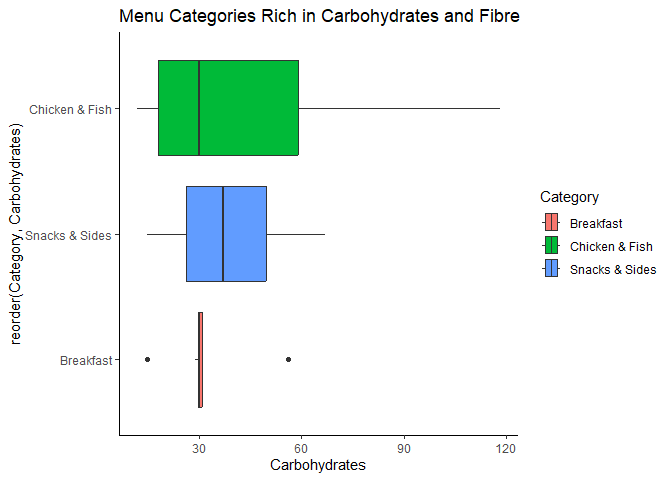
\includegraphics{index_files/figure-latex/unnamed-chunk-13-1.pdf}

\hypertarget{the-menu-categories-grouped-by-sodium-content}{%
\subsubsection{The Menu Categories grouped by sodium
content}\label{the-menu-categories-grouped-by-sodium-content}}

\begin{center}\rule{0.5\linewidth}{0.5pt}\end{center}

Our bodies need sodium; however, there is so much in most processed
foods, and too much sodium can have several negative effects. Canned
foods are notorious for having lots of sodium, as are bottled sauces,
salty snacks, and processed foods. Most nutritionists recommend watching
your sodium intake carefully because too much sodium in your diet is
dangerous. It can lead to high blood pressure and many related health
conditions.

\begin{center}\rule{0.5\linewidth}{0.5pt}\end{center}

\begin{Shaded}
\begin{Highlighting}[]
\NormalTok{sodium  }\OtherTok{\textless{}{-}}\NormalTok{ menu }\SpecialCharTok{\%\textgreater{}\%}
  \FunctionTok{select}\NormalTok{(Category,}
\NormalTok{         Item,Sodium,}
\NormalTok{         Sodium....Daily.Value.) }\SpecialCharTok{\%\textgreater{}\%} 
  \FunctionTok{group\_by}\NormalTok{(Category)}


\NormalTok{sodium\_plot }\OtherTok{\textless{}{-}}\NormalTok{ sodium }\SpecialCharTok{\%\textgreater{}\%} 
  \FunctionTok{ggplot}\NormalTok{(}\FunctionTok{aes}\NormalTok{(Sodium,}
\NormalTok{             Category,}
             \AttributeTok{fill =}\NormalTok{ Category)) }\SpecialCharTok{+}
  \FunctionTok{geom\_boxplot}\NormalTok{() }\SpecialCharTok{+} \FunctionTok{theme\_classic}\NormalTok{() }\SpecialCharTok{+} \FunctionTok{ggtitle}\NormalTok{(}\StringTok{"Menu Categories grouped by sodium content"}\NormalTok{)}


\NormalTok{sodium\_plot}
\end{Highlighting}
\end{Shaded}

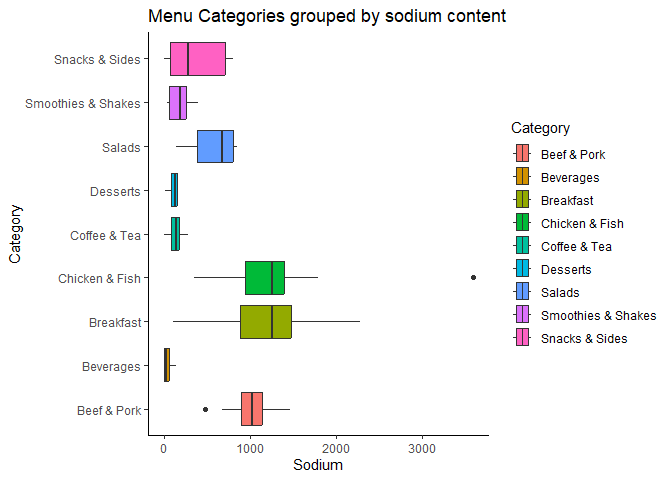
\includegraphics{index_files/figure-latex/unnamed-chunk-14-1.pdf}

\hypertarget{the-menu-categories-grouped-by-trans-fat}{%
\subsubsection{The Menu Categories grouped by Trans
Fat}\label{the-menu-categories-grouped-by-trans-fat}}

\begin{center}\rule{0.5\linewidth}{0.5pt}\end{center}

In the United States, the main dietary source of trans fats is partially
hydrogenated vegetable oils, previously used in many commercially
prepared foods. Consuming trans fats may adversely affect cholesterol
levels in the body and may contribute to the risk of atherosclerosis.
Because of this, the US Food and Drug Administration (FDA) has banned
the use of trans fats in prepared foods.

\begin{center}\rule{0.5\linewidth}{0.5pt}\end{center}

\begin{Shaded}
\begin{Highlighting}[]
\NormalTok{trans\_fat }\OtherTok{\textless{}{-}}\NormalTok{ menu }\SpecialCharTok{\%\textgreater{}\%}
  \FunctionTok{select}\NormalTok{(Category,}
\NormalTok{         Trans.Fat) }\SpecialCharTok{\%\textgreater{}\%}
  \FunctionTok{group\_by}\NormalTok{(Category)}

\NormalTok{trans\_plot }\OtherTok{\textless{}{-}}\NormalTok{ trans\_fat }\SpecialCharTok{\%\textgreater{}\%} 
  \FunctionTok{ggplot}\NormalTok{(}\FunctionTok{aes}\NormalTok{(Trans.Fat,}
\NormalTok{             Category,}
             \AttributeTok{fill =}\NormalTok{ Category)) }\SpecialCharTok{+} 
  \FunctionTok{geom\_boxplot}\NormalTok{() }\SpecialCharTok{+} \FunctionTok{theme\_classic}\NormalTok{() }\SpecialCharTok{+}  \FunctionTok{ggtitle}\NormalTok{(}\StringTok{"Menu Categories grouped by trans\_fat content"}\NormalTok{)}

\NormalTok{trans\_plot}
\end{Highlighting}
\end{Shaded}

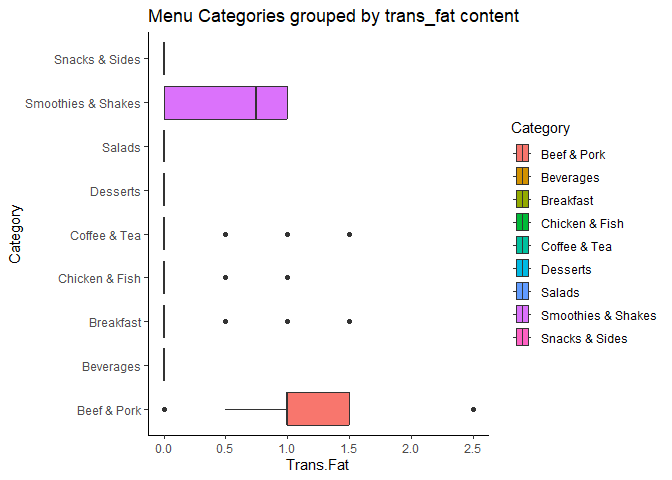
\includegraphics{index_files/figure-latex/unnamed-chunk-15-1.pdf}

\hypertarget{the-correlation-between-proteincarbohydrates-fat-and-calories}{%
\subsubsection{The Correlation between Protein,Carbohydrates, Fat and
Calories}\label{the-correlation-between-proteincarbohydrates-fat-and-calories}}

\begin{center}\rule{0.5\linewidth}{0.5pt}\end{center}

Fats are the slowest source of energy but the most energy-efficient form
of food.Because fats are such an efficient form of energy, the body
stores any excess energy as fat.

\begin{center}\rule{0.5\linewidth}{0.5pt}\end{center}

\begin{Shaded}
\begin{Highlighting}[]
\NormalTok{calories }\OtherTok{\textless{}{-}}\NormalTok{ menu }\SpecialCharTok{\%\textgreater{}\%}
  \FunctionTok{select}\NormalTok{(Calories,}
\NormalTok{         Carbohydrates, }
\NormalTok{         Protein,}
\NormalTok{         Total.Fat) }\SpecialCharTok{\%\textgreater{}\%} 
  \FunctionTok{group\_by}\NormalTok{(Calories)}

\NormalTok{calories\_plot }\OtherTok{\textless{}{-}} \FunctionTok{ggcorr}\NormalTok{(calories,}
       \AttributeTok{method =}  \FunctionTok{c}\NormalTok{(}\StringTok{"everything"}\NormalTok{, }\StringTok{"pearson"}\NormalTok{),}
       \AttributeTok{label =} \ConstantTok{TRUE}\NormalTok{)  }\SpecialCharTok{+} \FunctionTok{theme\_classic}\NormalTok{() }\SpecialCharTok{+}  \FunctionTok{ggtitle}\NormalTok{(}\StringTok{"Correlation of Calories and Macro{-}Nutrients"}\NormalTok{)}

\NormalTok{calories\_plot}
\end{Highlighting}
\end{Shaded}

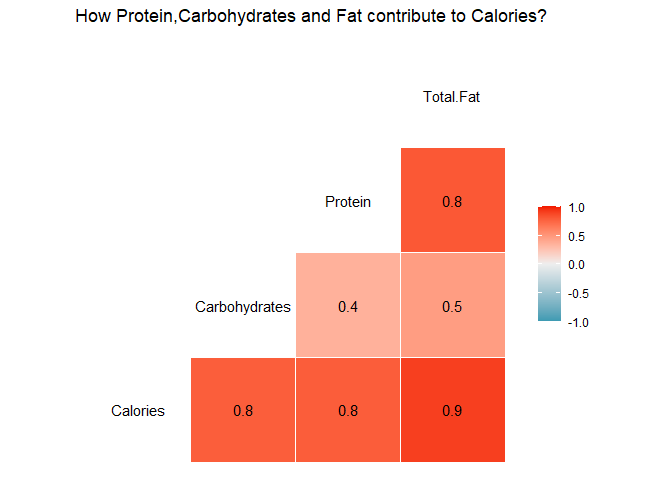
\includegraphics{index_files/figure-latex/unnamed-chunk-16-1.pdf}

\end{document}
